\chapter{面向仿冒应用的收集框架\mytool}
\label{chp:fakerevealer}

\section{设计缘由}
鉴于目前学术界中未有相关工作能提供仿冒应用的相关数据集,本研究需要率先尝试从工业界中系统地收集所需的仿冒应用数据。
然而,传统的网络爬虫框架只能机械、不加区分地爬取数据,不能具有针对性地爬取与本研究中的目标应用相关的样本;应用市场中应用数量太多,完全收集并不可行。
为了解决这个问题,本研究提出了面向仿冒应用的收集框架\mytool,创新地采用启发式的方法搜索与爬取与目标应用相关的样本,为后文的两项研究服务。

\section{应用收集流程简介}
仿冒应用是一个跟正版应用相对的概念,所以本文需要先定义正版应用,再根据正版应用的信息搜寻仿冒应用。

1)\ \emph{正版应用收集} \quad
在定义正版应用方面,本研究参考了数据平台易观千帆的月度App排行榜\footnote{\url{https://qianfan.analysys.cn/refine/view/rankApp/rankApp.html}},然后从中选出了其中的前50款热门App作为本次研究的目标App。
之后,笔者手动地从这50款App的官方网站上下载了这些应用的最新版本,作为正版应用的参考版本。

2)\ \emph{仿冒应用收集} \quad
要获取足量的仿冒应用数据以组成数据集是一个十分具有挑战性的任务,难点如下:
\begin{itemize}
	\item 要从多个不同的应用市场中爬取App样本,但每个应用市场都有不同的网页编码,不存在一个爬虫脚本对所有应用市场数据都通用的场景;
	\item 各个应用市场架上的App数量浩如繁星,需要有效地找到和目标App有关的所有样本,不重不漏;
	\item 对于大量数据,需要一个轻量级的解决方案快速判断获得的App样本究竟为正版应用又或者是仿冒应用。
\end{itemize}

为了应对第一个挑战,本研究与工业界合作,利用犇众信息公司的Janus平台对各大应用商店进行样本爬取,从而获得大量应用样本。
事实上,如\autoref{fig:Janus-data}显示,Janus平台自2017年起就开始对各大应用商店的App进行样本收集,至今已收集到上千万个App样本。
除样本搜集外,Janus也提供按规则搜索功能,用户可以创建自己的规则过滤平台中的应用数据,以获取自己需要的App样本。

\begin{figure}[htbp]
	\centering
	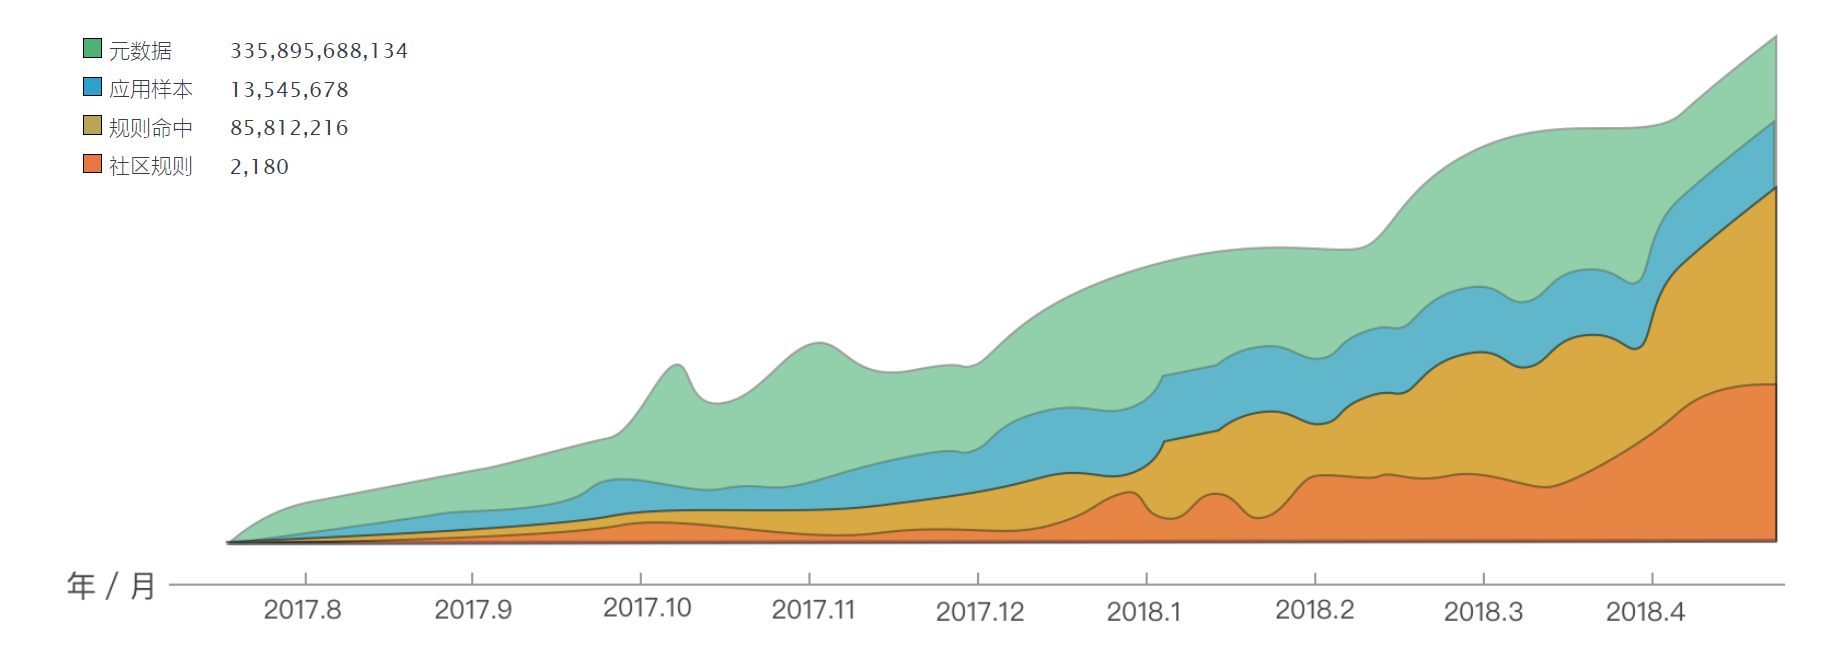
\includegraphics[width=\textwidth]{./Figures/edwin-Janus-data.png}
	\caption{Janus平台上的数据规模时序图}
	\label{fig:Janus-data}
	\vspace{-5mm}
\end{figure}

为了应对第二个和第三个挑战,本研究搭建了面向仿冒应用的收集框架\mytool。
% 利用一个基于广度优先搜索(Breadth-First Search,简称BFS)的算法,笔者在\mytool 中实现了一个\componentB ,以应用的\emph{包名}和\emph{应用名}作为拓展数据项,从Janus平台中分步迭代搜索与目标应用相关的所有App样本,然后将相关样本下载到本地保存;
% 对下载到本地的应用,笔者使用\mytool 的组件\componentA 提取所需的数据;
% 然后,基于前述收集到的正版应用信息,笔者在\mytool 中构建出了一个\componentC ,将上一步中提取到的数据和正版应用作比对。


\section{\mytool 的设计与实现}

本文使用Python 3开发了仿冒应用收集框架\mytool,该框架由\componentA 、\componentB 和\componentC 三个组件组成,\autoref{fig:FakeRevealer}展示了\mytool 的整体流程图。
输入初始正版应用的信息,\mytool 在经过迭代搜索、样本下载、应用过滤三个步骤之后,以CSV文件和JSON文件的形式输出仿冒应用各数据项和拓展后的正版应用信息。

\begin{figure}[htbp]
	\centering
	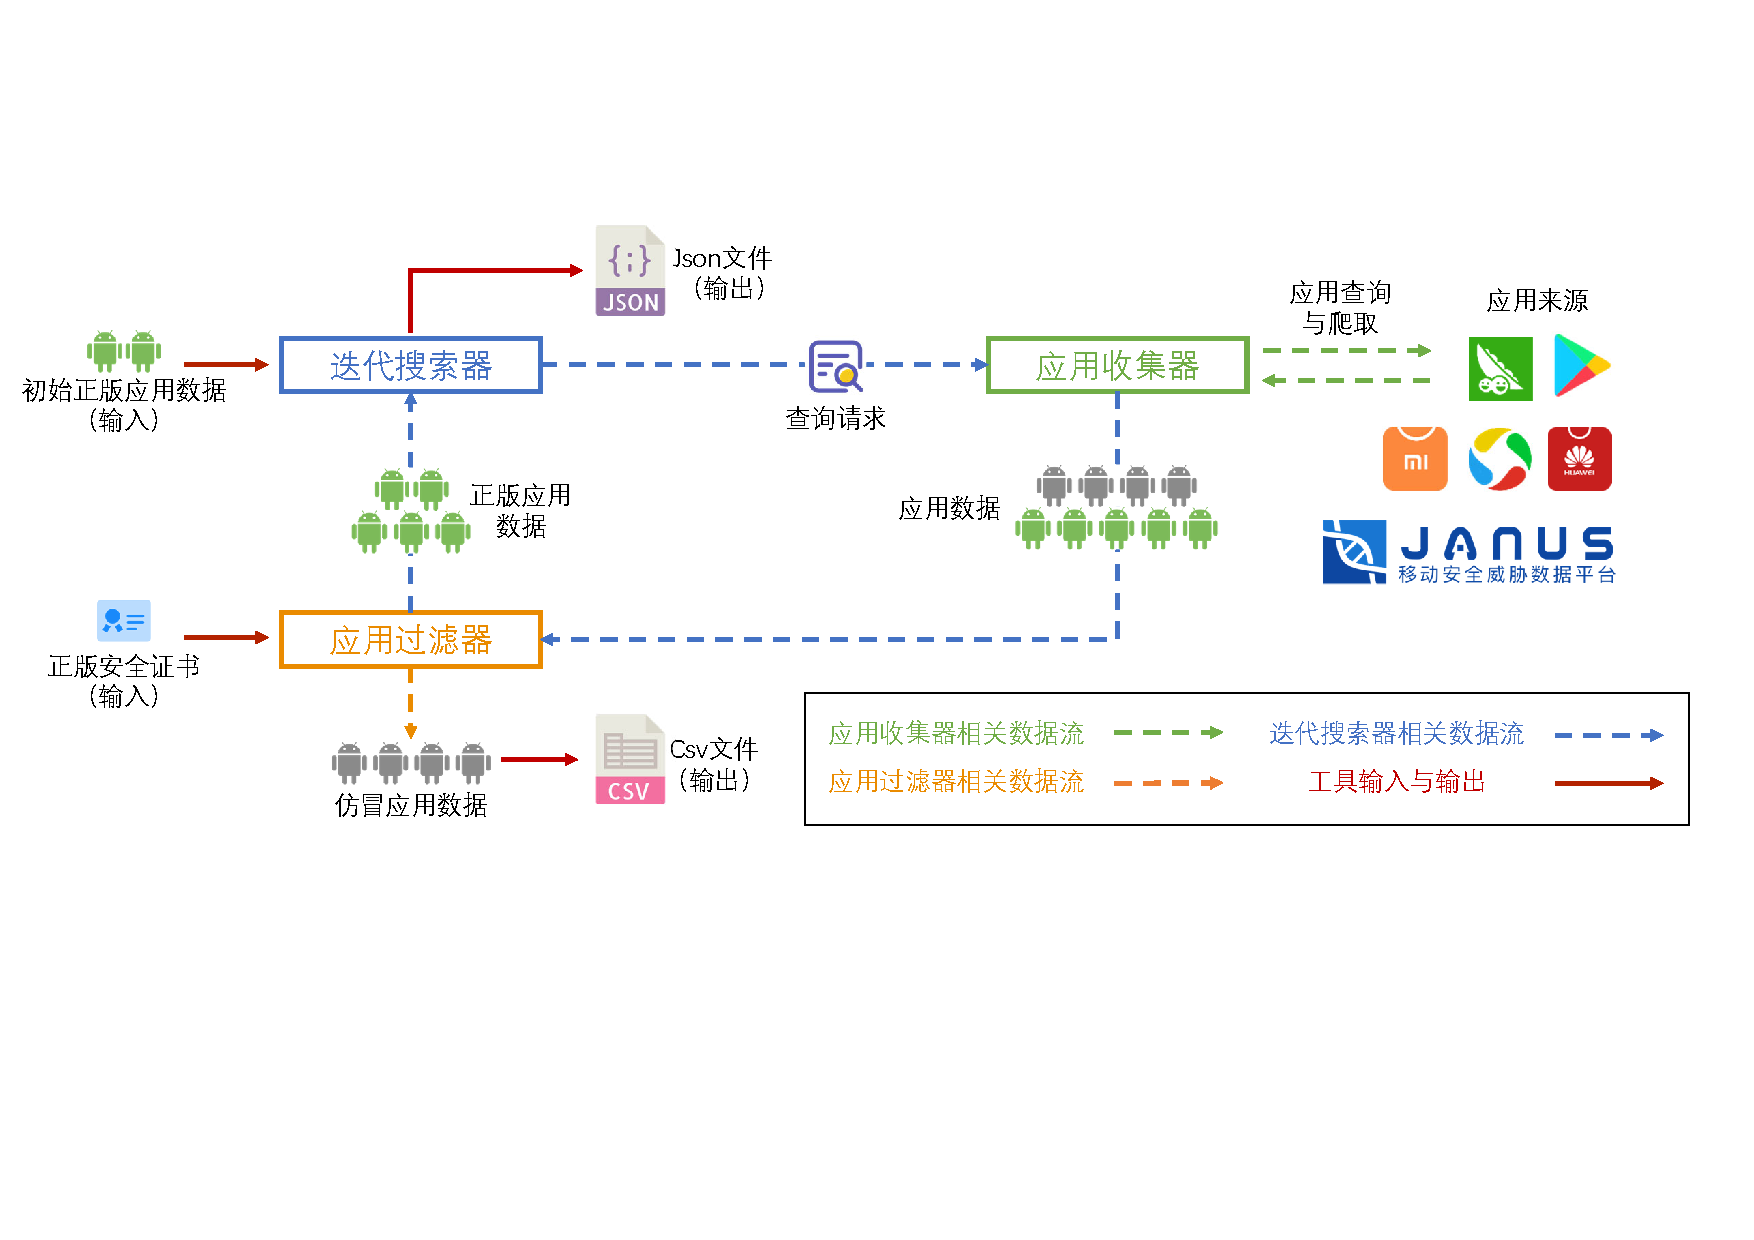
\includegraphics[width=\textwidth]{./Figures/edwin-fakerevealer}
	\caption{\mytool 整体结构}
	\label{fig:FakeRevealer}
	\vspace{-3mm}
\end{figure}

\subsection{\componentA }
\componentA 是与应用来源直接交互的部分,分为两个不同的子模块,分别是网络爬虫模块和APK包预处理模块。
在接收到应用收集请求之后,\componentA 会先根据收集请求,利用网络爬虫模块下载应用,然后再用APK包预处理模块对下载完毕的APK包提取信息,方便后续操作。

1)\ \emph{网络爬虫模块} \quad
本模块负责接收\componentA 的输入,根据输入中的需求从应用来源中查询并下载对应的App。
由于Janus平台上已经有提前收集好的源于各个应用市场的App样本,笔者直接从Janus上爬取应用。

不同应用商店提供应用查询、下载的API不同,不存在可以对应所有应用市场的爬虫脚本。
但只要能分析出应用商店查询、下载API的名称和用法,结合应用商店账户的Cookies,也能从商店中下载应用。
考虑到这个方面,笔者开发了插件化的爬虫模块。
针对不同的应用商店,使用者可以在使用网络包分析工具(如Burpsuite~\cite{burpsuite})解析到API与Cookies信息之后,将对应API和Cookies写入配置插件,再对网络爬虫模块配置对应当前商店的插件,开始爬取应用。

在具体实现方面,笔者利用Python自带的urllib库实现对网络资源的访问;由于下载是可以并发进行的事务,为了能提高运行效率,笔者利用了threading库对网络爬虫模块提供了多线程特性。

2)\ \emph{APK包预处理模块} \quad
这个模块负责从下载完毕的APK包中提取指定的数据项,存入键值对中,最后将所有应用的数据键值对以列表形式返回,作为\componentA 的输出。
APK文件中虽然包含着应用的所有信息,但本研究中的应用筛选并不需要用到整个APK文件,所以本模块会把筛选需要用到的数据先提取出来,后续处理时直接调用与该APK包有关的数据即可。
同时,由于不同APK包的大小不一,所需下载时长也各异,本框架在较大的应用还在下载的同时,对已经下载完毕的APK提取信息。
比起让\componentA 直接返回下载完毕的APK包、待后续需要数据时再进行数据提取的方法,这样的设计可以减小内存占用,也提高了框架的运行效率。

具体实现方面,APK包预处理模块使用Python的os库实现对命令行指令的调用,然后利用Android SDK中自带的命令行工具aapt对APK包进行解析,获取指定的数据项。


\subsection{\componentB }
这个组件的设计利用了一个基于广度优先搜索(Breadth-First Search,简称BFS)的算法,详情可见\autoref{alg:bfs}。
根据缓存中的正版应用信息,本组件向\componentA 提交查询、下载样本的请求。
在利用\componentC 过滤获得的应用信息后,再根据其中正版应用的信息扩增缓存中的数据,进行下一轮迭代搜索。

\begin{algorithm}[!ht]
	\tablewuhao
	\caption{迭代搜索算法}
	\label{alg:bfs}
    \KwIn{ $targetItems$,列表,用于拓展的数据项}
    \KwIn{ $legalApkInfo$,列表,包含正版应用及其信息键值对}
	\KwOut{ $cache$,列表,缓存拓展后的正版应用信息键值对}
	\SetKwProg{Fn}{Function}{:}{}

	\Fn {iterSearcher($legalApkInfo, targetItems$)} {

        $wtQueue$ = $\emptyset$;

        $cache$ = $\emptyset$;

        \For {$apkInfo \in legalApkInfo$} {

            \For {$item \in targetItems$} {

                $wtQueue$.add(${item: apkInfo[item]}$);

            }

        }

    	\While {$wtQueue \ne \emptyset$} {

    		$key, val$ = $wtQueue$.pop();

    		\If{${key: val} \in cache$} {continue;}

    		$cache$.add(${key: val}$);

    		$newSamples \gets$ appRetriever($key, val$);

    		\For {$sample \in newSamples$} {

                $isLegal \gets $ FakeFilter($sample$).getResult();

    			\If {$isLegal$} {

    				$sampleInfo \gets sample$.getInfo();

    				\For {$item \in targetItems$} {

    					$wtQueue$.add(${item: sampleInfo[item]}$);

    				}

    			}

    		}

    	}

    \KwRet{$cache$};

    }

\end{algorithm}

\autoref{alg:bfs}的输入有两项,分别是已有的正版应用信息列表$legalAppInfo$和要用来拓展搜索范围的数据项$targetItems$。

算法开始前,本框架先遍历每个正版应用的信息,将每个要拓展搜索的数据项对应的内容$apkInfo[item]$插入到待查询队列$wtQueue$中,完成初始化(第4 - 6行)。
然后是迭代搜索应用。
每次迭代中,本算法都从$wtQueue$中取出一组键值对,其中键$key$为本次迭代中用于搜索新应用的数据项,$val$为数据项对应的值(第8行)。
取出键值对之后,算法先检查该键值对是否已经被用于之前的搜索中。
如果该键值对之前已经出现过,就跳过本轮迭代,重新取一组键值对进行搜索;
否则,将本组键值对放入数据缓存$cache$,表示该组键值对已被使用过。
之后,组件将键值对传递给\componentA ,\componentA 会生成对应查询,从应用来源中获取数据项相关的应用(第12行)。
对于\componentA 返回的应用集$newSamples$中的每个样本$sample$,本文会用\componentC 检查$sample$是否为正版样本。
如果是正版样本,那么本算法将从该样本中获取对应的数据$sampleInfo$,然后将其中与待拓展对应项$item$对应的内容插入到待查询队列$wtQueue$中(第15 - 18行)。
当应用集$newSamples$中的所有样本都被筛选检查过之后,本轮迭代结束。
如果$wtQueue$中的所有键值对都已经被检索完毕(即$wtQueue$为空),本算法流程结束,本组件会将$cache$中被用于拓展搜索的各个数据项键值对整理成JSON文件输出,方便之后的再利用。

在本次实证研究场景中,$targetItems$包含两项内容,一个是应用的包名(\emph{PackageName}),另一个是应用自身的名字(\emph{AppName})。
之所以要这样操作,是因为开发者推出的App的应用名和包名并不是一成不变的。
一些热门应用会出于商业原因频繁地更改自己的应用名(比如爱奇艺视频,会根据其近期热播的电视剧/电影变更其应用名以吸引更多用户使用);
也有个别的热门应用可能会更换自己的包名,比如App有重大改版、又或者是开发者安全证书有变更,开发者不得不更换包名(具体原因可参考\secref{sec:signature}的Android App签名机制部分)。

\subsection{\componentC }
顾名思义,\componentC 的功能是从输入的应用程序集之中将仿冒应用筛选出来,其核心是安全证书的识别。
根据\secref{sec:signature}中对Android应用签名机制的描述,一个App中包含的安全证书文件指示了对APK文件进行修改的开发者。
如果一个APK文件中包含的安全证书信息与指定应用的开发者信息相符,那么本组件认为这个APK包来源于正版的开发者;否则本组件认为这是一个仿冒应用。

在开始过滤之前,开发者需要先向过滤器导入正版证书信息。
之后,对于每个输入的应用,组件会将其安全证书信息和正版证书信息作比对。
对于证书信息相符的应用,本组件会将其放入\componentB 的待检索队列中用作下一轮的迭代搜索;
而证书信息不相符的应用则会被筛选出并保存。

在迭代搜索的流程结束之后,本组件会将保存的所有仿冒应用数据项导出成CSV文件保存,方便之后的数据挖掘。


\section{仿冒应用数据概览}
以下是框架收集到的数据的概览:

从易观千帆提供的数据榜单中,本研究选择了50个最热门的App作为目标App,这些App分属11个不同的应用类别。
由于App的应用名可能会在App更新迭代的时候随之变更,笔者用基于BFS的策略,从50种App中一共记录了198个不同的应用名,来挖掘仿冒样本。

在这50款App中,以下三款App的样本并不能在市面上找到:\emph{OPPO 应用商店},\emph{华为应用商店}和\emph{小米应用商店}。
因为这三款App都是由手机设备厂商开发和预装在对应品牌的手机中的,仅供这些品牌的用户使用,并不在其他应用市场上提供下载。
当然,这也是这三款App热度高的原因——这几款App都被预装到了对应手机品牌厂商的每一部Android设备中,而OPPO、华为和小米又是国内最大的几家手机厂商,这几款App自然也会有庞大的用户基数。
因此,本研究最后的目标App只有47款。

对这47款目标App,笔者总共收集到了138,106个应用样本。
其中,69,614个应用样本持有官方开发者证书,52,638个应用样本并不具有官方证书。
还有一部分应用样本,是某些应用的分别发布在不同应用市场同一版本,在经过去重筛选后被排除(共计15,854个)。

对于每个样本,框架收集8个数据项作为元数据:\emph{样本SHA1码},\emph{安全证书SHA1码},\emph{包名},\emph{样本大小},\emph{版本号},\emph{搜集时间}和\emph{APK包来源}。
其中,\emph{样本SHA1码}是使用SHA1哈希算法对整个APK文件进行数据摘要之后获取到的编码串,每个样本都有独一无二的SHA1码;安全证书SHA1码则是对样本的安全证书采用SHA1算法提取数据摘要之后获取的编码串,用于识别不同的证书。
而\emph{搜集时间}则是样本从应用市场被爬取到数据库的时间点,\emph{APK包来源}指示该APK包来源的应用市场。


\section{本章小结}
本章介绍了数据收集的流程和方法,然后讲述了面向仿冒应用的收集框架\mytool 的工作流程,以及其中三个组件——\componentA 、\componentB 和\componentC 的设计实现,最后对采集到的数据进行了简要描绘。

尽管\mytool 在设计之时选择了利用包名和应用名迭代搜索、通过安全证书筛选的机制过滤仿冒应用,但框架本身的流程并不囿于此机制中,读者可以参考本框架流程,设计其他过滤仿冒应用,或者是其他任何具有某种特征的应用的工具。

在明确数据收集流程之后,本研究针对仿冒样本中采集到的元数据进行了挖掘分析,以求获得对于仿冒应用生态和特征、以及对于仿冒应用开发者的行为的更全面的认知。
